The discovery of the Higgs boson~\cite{Aad:2012tfa,Chatrchyan:2012ufa}
and extensive searches for signals of new physics at the LHC impose
conditions on the precision of the Standard Model (SM) predictions for
hard scattering processes in hadron-hadron collisions.
%\\
%% old proposal:
%In the era of the Higgs discovery~\cite{Aad:2012tfa,Chatrchyan:2012ufa} and extensive searches
%for signals of new physics at the LHC it is crucial
%to have accurate Standard Model (SM) predictions for
%hard scattering processes in hadron-hadron collisions.
The most common approach to calculate the SM cross sections for  
such reactions is to use collinear factorisation in perturbative QCD (pQCD)~\cite{Collins:1989}:
%{\small
\begin{equation}
\small
\begin{array}{lcl}
\sigma(\as,\mur,\muf) & = &
\sum\limits_{a,b}\,  \int\limits_{0}\limits^{1} dx_1\ dx_2\, f_a(x_1,\as,\muf) 
 f_b(x_2,\as,\muf)\\ 
& \times & \, \hat{\sigma}^{ab}(x_1,x_2;\as,\mur,\muf).
\label{eq:fact}
\end{array}
\end{equation}
%}
Here the cross section $\sigma$ for 
%inclusive Higgs production
any hard-scattering inclusive process $ab \rightarrow X + all$
is expressed
as a convolution of Parton Distribution Functions (PDFs) $f_a$ and $f_b$
with the partonic cross section
% that describe
%the 
%$\hat{\sigma}^{ab \rightarrow H + X}$.
$\hat{\sigma}^{ab}$.
%
The PDFs represent 
the probability of finding a specific parton $a$ ($b$) in the first (second) proton carrying a fraction $x_1$ ($x_2$) of its momentum.
%
Indices $a$ and $b$ in the Eq.~\ref{eq:fact} indicates the various 
kinds of partons,
i.e. gluons, quarks and antiquarks of different flavours, 
that are considered
as the constituents of the proton.
%
Both the PDFs and the partonic cross section depend on the strong coupling
$\as$, and the factorisation and renormalisation scales,
$\muf$ and $\mur$, respectively.
%
The partonic cross sections are calculable in pQCD whereas
PDFs cannot be computed analytically in QCD,
they must rather be determined from measurement. 
%
PDFs are assumed to be universal such that different scattering reactions can be used 
to constrain them~\cite{Perez:2012um,Forte:2013wc}.
% in particular one can use specific reaction data 
%for determining the PDFs and then use these PDFs for
%predicting other processes.
%

Measurements of the inclusive Neutral Current (NC) and Charged Current (CC)  
Deep-Inelastic-Scattering (DIS) at the $ep$ collider HERA provide crucial information for determining the PDFs.
%
For instance, the gluon density relevant
for calculating the dominant gluon-gluon fusion contribution to Higgs production
at the LHC can be accurately determined at low and medium $x$ solely from the HERA data.
%
Many processes in $pp$ and $p \bar p$ collisions at LHC and Tevatron, respectively, 
probe PDFs in the kinematic ranges, complementarly to the DIS measurements. 
Therefore inclusion of the LHC and Tevatron data in the QCD analysis of the proton structure 
provide additional constraints on the PDFs, improving either their precision, 
or providing important information of the correlations of PDF with the fundamental 
QCD parameters like strong coupling or quark masses. 
%
%Despite being often plagued by larger perturbative uncertainties,
%
In this context, the processes of interest at hadron colliders are
Drell Yan (DY) production, $W$ asymmetries, associated production of $W$ or $Z$ bosons 
and heavy quarks, top quark, jet and prompt photon production.
%

%\fitter~represents a QCD analysis framework that aims at 
%determining precise PDFs by integrating all the PDF sensitive information
%from HERA, the Tevatron and the LHC.
%
The open-source QCD platform \fitter encloses the set of tools  necessary for a comprehensive global 
QCD analysis of hadron-induced processes even at the early stage of the experimental measurement. 
It has been developed for determination of PDFs and extraction of fundamental QCD parameters such as the heavy
quark masses or the strong coupling constant. This platform also provides the basis for 
comparisons of different theoretical approaches and can be used for direct tests of the impact 
of new experimental data in the QCD analyses.
%
The processes that are currently available in \fitter framework are listed in Tab.~\ref{tab:proc}.
%
\begin{table}
\small
%\tiny
\scriptsize

\begin{tabular}{|l|l|l|l|}
\hline 
\textbf{Data} &\textbf{Process}&\textbf{Reaction}&\textbf{Theory} \\
        &     &               &\textbf{calculations, schemes}  \\
\hline \hline \\ [-2.5ex]
%\multirow{6}{*}{HERA} &DIS NC   &$ep\to eX$      & TR', ACOT \\
HERA &DIS NC   &$ep\to eX$      & TR', ACOT \\
     &         &                & ZM (\qcdnum) \\
     &         &                & FFN (\texttt{OPENQCDRAD}, \\
     &         &                & \qcdnum), \\ 
     &         &                & TMD (uPDFevolv) \\ [0.5ex]
\cline{2-4}  \\ [-2.0ex]
     &DIS CC   &$ep\to \nu_e X$ & ACOT, ZM (\qcdnum) \\
     &         &                & FFN (\texttt{OPENQCDRAD)} \\  [0.5ex]
\cline{2-4}  \\ [-2.0ex]
     &DIS jets &$ep\to e\ \mathrm{jets}$      & \nlojetpp (\fastnlo)\\ [0.5ex]
\cline{2-4} \\ [-2.0ex]
     &DIS heavy quarks & $ep\to e c \bar{c} X$, & ZM (\qcdnum), \\
     &         & $ep\to e b \bar{b} X$ & TR', ACOT, \\
     &         &                & FFN (\texttt{OPENQCDRAD}, \\
     &         &                & \qcdnum) \\  [0.5ex]
\hline \\ [-2.5ex]
Fixed Target   &DIS NC          &$ep\to eX$ & ZM (\qcdnum), \\
     &         &                & TR', ACOT \\ [0.5ex]
\hline \\ [-2.5ex]
Tevatron, LHC &Drell Yan &$pp(\bar p)\to l\bar l X$, & \mcfm (\applgrid) \\
              &          &$pp(\bar p)\to l\nu  X$ &                 \\ [0.5ex]
\cline{2-4}  \\ [-2.0ex]
%Tevatron, LHC &W charge asym &$pp(\bar p) \to l\nu X$ & MCFM (\texttt{APPLGRID}) \\
%\hline
              &top pair   &$pp(\bar p) \to t\bar t X$  & \mcfm (\applgrid),  \\
              &            &                            & \texttt{HATHOR}      \\  [0.5ex] 
\cline{2-4}  \\ [-2.0ex]
              &single top &$pp(\bar p) \to t l \nu X$,      & \mcfm (\applgrid) \\
              &           &$pp(\bar p) \to tX$,             &  \\
              &           &$pp(\bar p) \to tWX$             &  \\ [0.5ex]
\cline{2-4}  \\ [-2.0ex]
             &jets &$pp(\bar p) \to \mathrm{jets} X$ & \nlojetpp (\applgrid), \\
                &  & & \nlojetpp (\fastnlo) \\ [0.5ex]
\hline  \\ [-2.5ex] 
LHC& DY+heavy quarks &$pp \to VhX$ & \mcfm (\applgrid) \\  [0.5ex]
\hline
\end{tabular}
\caption{The list of processes available in the \fitter package. 
The refernces for the individual calculations and their implementations are given in the text.
}
%The APPLGRID~\cite{Carli:2010rw} and FastNLO~\cite{Kluge:2006xs,Wobisch:2011ij,Britzger:2012bs} 
%techniques for the fast interface to theory calculations are described in section~\ref{sec:techniques}.} 
\label{tab:proc}
\end{table}
%
\normalsize
The functionality of \fitter is schematically illustrated in Fig.~\ref{fig:flow} and it can be divided in four main blocks: %{\bf needs to update figure!}
\begin{figure}[!ht]
  \begin{tikzpicture}[node distance=1cm, auto,>=latex', thick]
      \path[->] node[draw, text width=2cm, align=center] at (0,0) (init) {\bf Initialization};
      \path[->] node[draw, below left=0.3cm and -0.7cm of init, text width=3.5cm] (data) 
                    {\begin{center} \vspace{-0.3cm}{\bf Input Data} 
		      \\ {\color{blue}\small Data Type} 
		     \end{center} 
		     {\scriptsize 
		     \begin{itemize}
                      \vspace{-0.3cm}
		      \item Collider ep
		      \item Collider pp
		      \item Fixed target data
		     \end{itemize}}
		     } (init) edge (data);
      \path[->] node[draw, below right=0.3cm and -0.7cm of init, text width=3.5cm] (theory) 
                    {\begin{center} \vspace{-0.3cm}{\bf Theory Predictions} 
		      \\ {\color{red}\small Factorization Theorem} 
		     \end{center} 
		     {\scriptsize 
		     \begin{itemize}
                      \vspace{-0.3cm}
		      \item PDF Parametrisation
		      \item QCD Evolution (QCDNUM)
		      \item Cross Section Calculation
		     \end{itemize}}
		     } (init) edge (theory);
      \path[->] node[draw, below right=0.4cm and -1.4cm of data, text width=3.5cm] (minuit) 
                    {\begin{center} \vspace{-0.3cm}{\bf Minimisation (MINUIT)} 
                      \vspace{-0.2cm}
		     \end{center} 
		     {\color{blue}\scriptsize Treatment of the uncertainties:} 
		     {\scriptsize 
                      \vspace{-0.1cm}
		     \begin{itemize}
		      \item PDF Parametrisation
		      \item QCD Evolution (QCDNUM)
		      \item Cross Section Calculation
		     \end{itemize}}
		     } (data) edge (minuit)
		     (theory) edge (minuit)
		     (data) ++ (1.6,0) edge [<->,double equal sign distance] ++(1.36,0) (theory);
      \path[->] node[draw, below =0.4cm  of minuit, text width=3.5cm] (res) 
                    {\begin{center} \vspace{-0.3cm}{\bf Results} 
		     \end{center} 
		     {\scriptsize 
		     \begin{itemize}
                      \vspace{-0.3cm}
		      \item PDF LHgrids
		      \item alphas, mc, \dots
		      \item Data vs Predictions
		      \item \(\chi^2\), pulls, shifts
		     \end{itemize}}
		     } (minuit) edge (res);
  \end{tikzpicture}
  \caption{Schematic structure of the \fitter program.} 
  \label{fig:flow}
\end{figure}

%\begin{figure}[!ht]
%   \centering
%   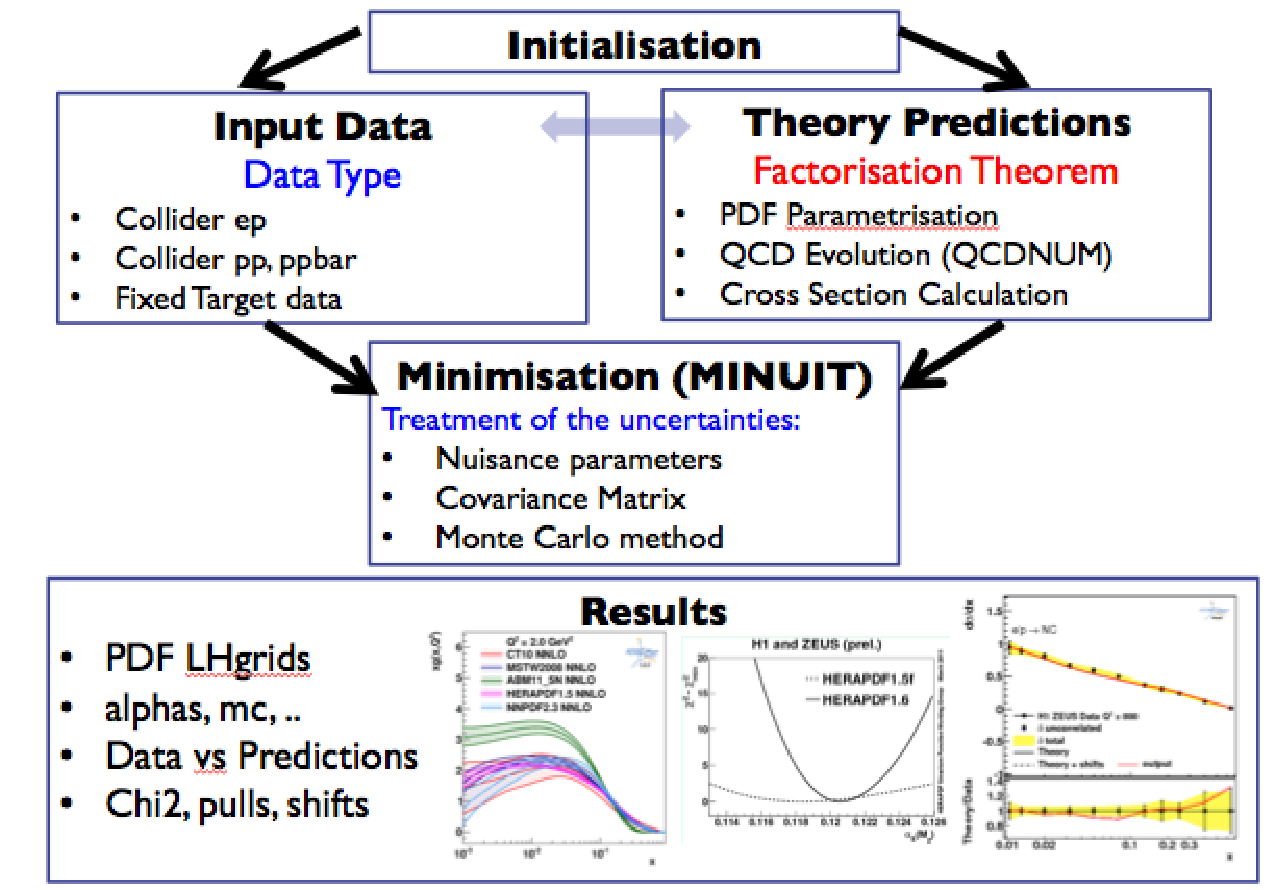
\includegraphics[width=8cm]{flow.pdf}
%   \caption{Schematic structure of the \fitter~program.} 
% \label{fig:flow}
%\end{figure}
\begin{description}
\item 
\bf {Input data:} \rm The relevant cross section measurements from the various processes
are stored internally in \fitter with the full information on their uncorrelated and correlated
uncertainties. HERA data sets are the basis of any proton PDF extraction, 
and they are used by all global PDF groups \cite{MSTWpdf, CT10pdf, NNPDFpdf, ABMpdf, JRpdf}. 
Additional measurements provide constraints to the sea flavour decomposition, such as the new 
results from the LHC, as well as constraints to PDFs in the kinematic phase-space regions 
where HERA data is not measured precisely, such as the high $x$ region for the gluon and valence quark distributions from Tevatron and fixed target experiments..
\item
\bf{Theory predictions:} \rm  Predictions for cross section of different processes are obtained using 
the factorisation approach (Eq.~\ref{eq:fact}). The PDFs are parametrised at a starting input scale $Q_0^2$  
by a chosen functional form with a set of free parameters $\vec{p}$. These PDFs are then evolved 
from $Q_0^2$ to the scale of the measurement using the 
Dokshitzer-Gribov-Lipatov-Altarelli-Parisi 
(DGLAP)~\cite{Gribov:1972ri, Gribov:1972rt, Lipatov:1974qm,
Dokshitzer:1977sg, Altarelli:1977zs} evolution equations 
(as implemented in \qcdnum~\cite{qcdnum}), 
CCFM \cite{\CCFM} or dipole models~\cite{Golec-Biernat:1998js,Iancu:2003ge,Bartels:2002cj} 
and then convoluted with the hard parton cross sections calculated
using a relevant theory program (as listed in Tab.~\ref{tab:proc}).
\item
\bf{QCD fit:} \rm  The PDFs are extracted from a least square fit by minimising the  $\chi^2$ function with respect to free parameters. The $\chi^2$ function is formed from the input data and the theory prediction.
The $\chi^2$ is  minimised iteratively 
with respect to the PDF parameters using the MINUIT~\cite{minuit} program.
Various choices of accounting for the experimental uncertainties are employed in \fitter, either using 
a nuisance parameter method for the correlated systematic uncertainties, 
or a covariance matrix method (see details in section~\ref{sec:chi2representation}). In addition, \fitter allows to study different statistics 
assumptions for the distributions of the systematic uncertainties (i.e. Gauss or log-normal)~\cite{hera-lhc:report2009}.
%
%In the $\chi^2$ minimisation,
%The parameters $\vec{p}$ of the parametrised PDFs and their uncertainties are extracted from the minimisation fit.
%Fitted values of $\vec{p}$ and estimated uncertainties are obtained.
%The fitted parameters $\vec(p)$ and obtained from the uncertainties of the parameters are determined (from chi2+1???)
%
\item
\bf{Results:} \rm 
%The fitted parameters $\vec{p}$ and their estimated uncertainties are produced. 
The resulting PDFs are provided in a format ready to be used by the \lhapdf 
library~\cite{lhapdf,lhapdfweb} or by \tmdlib \cite{tmdlref}.
\fitter drawing tools can be used to display the PDFs with the uncertainty at a chosen scale.  
%Drawing tools are supplied which allow the PDFs to be
%graphically  displayed at chosen scales by the users with their one sigma uncertainty bands. 
A first set of PDFs extracted by \fitter is HERAPDF1.0 \cite{h1zeus:2009wt}, shown in Fig.~\ref{fig:hera1}, 
which is based on HERA~I data.
Since then several other PDF sets were produced within the HERA and LHC collaborations.
In addition to the PDF display, 
the visual comparison of data used in the fit to the theory predictions are also produced. 
% plots which compare the input data to the fitted theory predictions can be produced 
%to demonstrate the fit consistency. 
\begin{figure}[!ht]
   \centering
   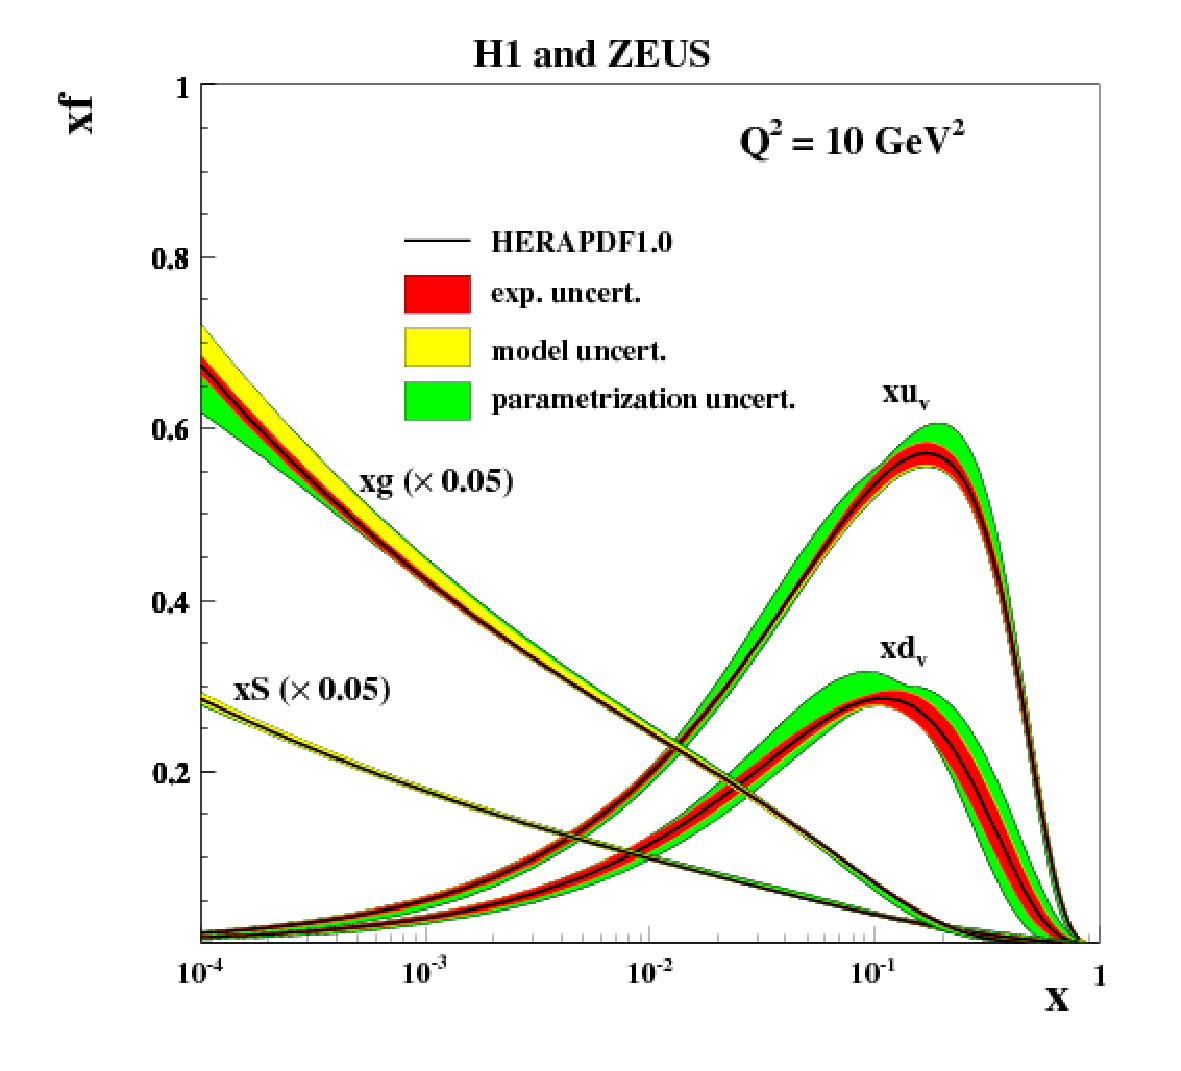
\includegraphics[width=8cm]{hera1.pdf}
   \caption{Summary plots of valence ($xu_v$, $xd_v$), total sea ($xS$, scaled) and gluon ($xg$, scaled) densities
   with their experimental, model and parametrisation uncertainties shown as colored bands at the scale 
   of $Q^2=10 \ \GeV^2$ for the HERAPDF1.0 PDF set at NLO~\cite{h1zeus:2009wt}.}
 \label{fig:hera1}
\end{figure}
In Fig.~\ref{fig:data}, a comparison of inclusive NC data from the HERA~I running period with predictions based on HERAPDF1.0. It also illustrates the comparison to the theory predictions which are adjusted by the  
systematic uncertainty shifts when using the nuisance parameter method that accounts for 
correlated systematic uncertainties. 
As an additional consistency check between data and the theory predictions, pull information, defined as the difference between data and prediction divided by the uncorrelated uncertaintly of the data, is displayed in units of sigma shifts for each given data bin.
% related only to the uncorrelated part of the systematic uncertainty. 

\begin{figure}[!ht]
   \centering
   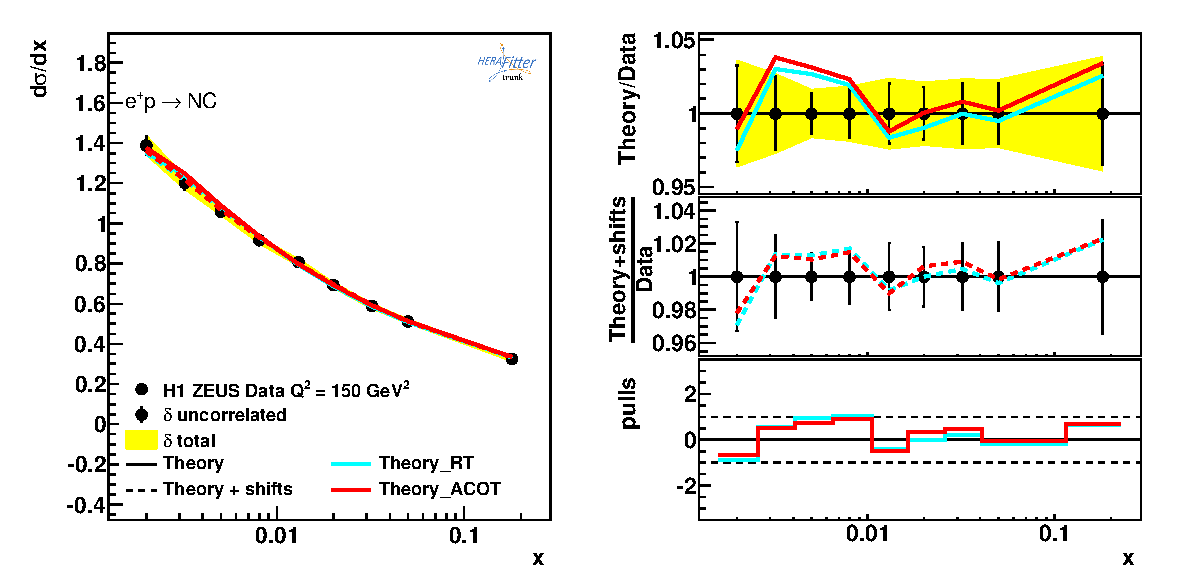
\includegraphics[width=8.6cm]{datatheory.pdf}
   \caption{An illustration of the \fitter drawing tools comparing the measurements (in the case of HERA I) to the predictions of the fit. In addition, ratio plots are also provided together with the pull distribution (right panel).} 
 \label{fig:data}
\end{figure}

\end{description}
%
%This paper provides a comprehensive description of  \\
%the \fitter\ package.
%which is designed for analysis of the High Energy Physics data.
%The package has been developed by members of the H1 and ZEUS collaborations
%with an exclusive support of different theoretical groups.
%The main purpose of the \fitter\ package is analysis of the 
%data from the $e^{\pm}p$, $p\bar{p}$, and $pp$ collider experiments
%information obtained from the deep inelastic scattering experiments
%and the determination of the parton density functions (PDFs).
%The broad range of data taken from the $e^{\pm}p$, $p\bar{p}$, and $pp$ collider experiments can be
%studied by the package. 

%Based on the concept of factorisable nature of the cross sections into universal parton distribution functions (PDFs) and process dependent partonic scattering cross sections, 

%The \fitter\ program facilitates the determination of the PDFs from many 
%cross section measurements at $ep$, $p\bar{p}$ or $pp$ colliders.  
% It includes various options for theoretical calculations and various choices 
%of how to 
%account for the experimental uncertainties. 
The \fitter project provides a versatile environment for benchmarking studies 
and a flexible platform for the QCD interpretation of analyses within the LHC experiments,
as already demonstrated by several publicly available results using the \fitter framework~\cite{atlas:strange,atlas:jets,atlas:hm,cms:strange,cms:jets,h1:2012kk,h1zeus:charm}.  

The outline of this paper is as follows.
%
Section~\ref{sec:theory} discusses the various processes 
and corresponding theoretical calculations performed in the DGLAP~\cite{Gribov:1972ri,Gribov:1972rt,Lipatov:1974qm,
Dokshitzer:1977sg,Altarelli:1977zs} formalism that are available in \fitter.
%
Section~\ref{sec:techniques} presents various techniques employed by the theory calculations used in \fitter.
Section~\ref{sec:method} elucidates the 
methodology of determining PDFs through fits based on various
% {\bf (what do you mean here
%by approaches?)} 
 $\chi^2$ definitions used in the
minimisation procedure. 
Alternative approaches to the DGLAP formalism are presented in section~\ref{sec:alternative}.
%
Specific applications of the package are given in
section~\ref{sec:examples} and the summary is presented in section~\ref{sec:summary}.
%
%{\bf add something more here?.}
